\section{机械振动}

\begin{proset}
    如图所示，物块静止在水平面上，绕过光滑定滑轮的细线一端连接在物块上，另一端连接轻弹簧，轻弹簧下面吊着小球，滑轮两边的细线竖直，物块及小球均处于静止状态，将小球缓慢下拉，当物块对地面的压力恰好为零，由静止释放小球，小球做简谐运动。已知小球上升到最高点时，弹簧恰好处于原长，重力加速度大小为\(g\)，则下列说法正确的是\paren[]

    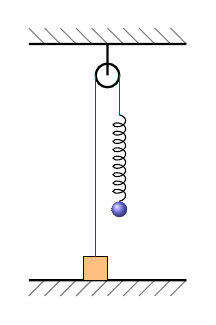
\begin{tikzpicture}
        \foreach \x in {-1,-.8,...,.8}
            {\draw[gray] (\x,-.2)--++(.2,.2);
            \draw[gray] (\x,3.2)--++(.2,-.2);}
        \draw[thick] (-1,0)--(1,0) (-1,3)--(1,3) (0,2.6) circle(.15) (0,2.6)--(0,3);
        \draw[fill=orange!50] (-.3,0) rectangle(0,.3);
        \draw[purple] (-.15,.3)--(-.15,2.6) (.15,2.6)--(.15,2.1);
        \draw[decoration={aspect=.6,segment length=3,amplitude=.8mm,coil},decorate] (.15,2.1)--(.15,1);
        \shade[ball color=blue!50] (.15,.9) circle(.1);
    \end{tikzpicture}
    \begin{choices}
        \item 释放小球瞬间，小球的加速度大小为\(g\)
        \item 释放小球瞬间，物块的加速度大小为\(g\)
        \item 物块的质量为小球的质量的3倍
        \item 小球向上运动过程中，重力势能和弹簧的弹性势能之和先增大后减小
    \end{choices}
\end{proset}
\begin{answer}
    A\quad 提示：小球做简谐运动，首先找到平衡位置，由释放位置到静止的位置关于平衡位置对称。
\end{answer}

\begin{proset}
    （多选）
    如图所示，倾角为\(\theta =\)\,\qty{30}{\degree}的足够长光滑绝缘斜面固定在水平面上，空间中存在水平向右的匀强电场，电场强度\(E = \frac{\sqrt{3}mg}{3q} \)。小球\(A\)的电荷量为\( + q\)(\(q > 0\))，小球\(B\)不带电，质量均为\(m\)，两球用劲度系数为\(k\)的轻质绝缘弹簧连接，弹簧处于原长并锁定。现解除锁定释放两球并开始计时，\(t_0\)时刻两球第一次速度相等，速度大小为\(v_0\)，此时弹簧形变量为\(x_0\)，在整个运动过程中弹簧均在弹性限度内，重力加速度为\(g\)。下列说法正确的是\paren[]

    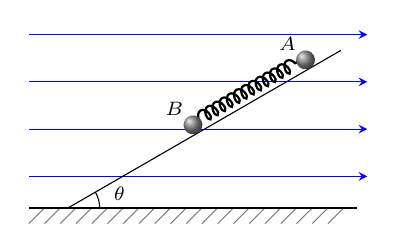
\begin{tikzpicture}[font=\scriptsize]
        \foreach \y in{.4,1,...,2.5}
            \draw[-stealth,blue] (-.5,\y)--(3.8,\y);
		\def\TheTa{30}%旋转角度
		\def\LenGth{4}%斜面长度
		\pgfmathsetmacro\CosLenGth{\LenGth*cos(\TheTa)}
		\begin{scope}[rotate=\TheTa]	
			\draw (0,0)--++(\LenGth,0);
            \draw[thick,decoration={aspect=.6,segment length=3,amplitude=.8mm,coil},decorate] (2,.15)--(3.5,.15);
            \shade[ball color=gray] (1.9,.12)node[above left,black]{\(B\)} circle(.12);
            \shade[ball color=gray] (3.55,.12)node[above left,black]{\(A\)} circle(.12);
		\end{scope}
		\draw (.4,0) arc(0:\TheTa:.4);
		\node at(.65,.18){\(\theta\)};
		\foreach \x in{-.5,-.3,...,\CosLenGth}
			\draw[gray] (\x,-.2)--++(.2,.2);
		\draw[thick] (-.5,0)--({\CosLenGth+.2},0);
	\end{tikzpicture}
    \begin{choices}
        \item 两球每次加速度相同时弹簧的形变量均为\(\frac{mg}{4k}\)
        \item 两球每次速度相同弹簧形变量均为\(x_0\)
        \item 在\(t = t_0\)时，小球\(A\)的电势能增加了\(\frac{mg}{8}(v_0t_0 - x_0)\)
        \item 在\(t = 2t_0\)时，两球和弹簧系统机械能减少了\(mgv_0t_0\)
    \end{choices}
\end{proset}
\begin{answer}
    AD\quad 提示：两球质心做匀加速运动，\(a_c = \frac{\frac{1}{2}mg}{2m} = \frac{1}{4}g\)
\end{answer}

\section{机械波}

\begin{proset}
    某仪器发射两列脉冲横波，在同一均匀介质中相向传播，波速\(v\)的大小均为\,\qty{2}{m/s}。\(t = 0\)时刻的波形图如图所示，此后波在传播的过程中，下列描述正确的是\paren[]

    \begin{tikzpicture}[font=\scriptsize,>=latex]
        \draw[->,blue] (-4.5,0)--(2.5,0)node[below]{\(x\)/\,\qty{}{m}};
        \draw[->,blue] (0,-.5)--(0,1.8)node[right]{\(y\)/ \,\qty{}{cm}};
        \foreach \x/\n in{-4/-8,-3/-6,-2/-4,-1/-2,1/2,2/4}
            \draw[blue] (\x,.1)--++(0,-.1)node[below]{\(\n\)};
        \draw[purple,domain=-4:-2,smooth] plot(\x,{1.2*sin(pi*\x/2 r)});
        \draw[purple,domain=1:2,smooth] plot(\x,{-.6*sin(pi*\x r)});
        \draw[dashed] (-3,0)--(-3,1.2)--(0,1.2)node[blue,right]{4} (1.5,0)--(1.5,.6)--(0,.6)node[blue,left]{2};
    \end{tikzpicture}
    \begin{choices}
        \item 在\(x =\) \,\qty{0}{m}处两列波相遇
        \item \(t =\) \,\qty{3}{s}两列波开始相遇
        \item \(t =\) \,\qty{2}{s}时\(x =\) \,\qty{-3}{m}质点的速度与加速度方向相反
        \item \(t =\) \,\qty{2.25}{s}时某个质点的位移能达到\,\qty{6}{cm}
    \end{choices}
\end{proset}
\begin{answer}
    D\quad 提示：两列波波峰相遇时振动加强\(t = \frac{3 -( - 6)} {4} =\) \,\qty{2.25}{s}
\end{answer}